\documentclass[border=5pt]{standalone}
\usepackage{tikz}
\usepackage{amsmath}
\begin{document}
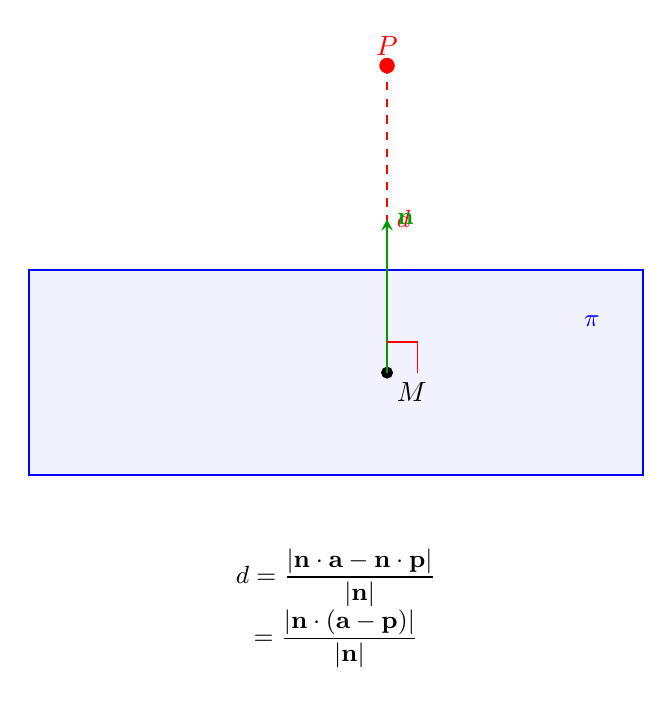
\begin{tikzpicture}[scale=1.3, >=stealth]
  % Distance from point to plane

  % Plane
  \fill[blue!10, opacity=0.5] (-3,-0.5) -- (3,-0.5) -- (3,1.5) -- (-3,1.5) -- cycle;
  \draw[thick, blue] (-3,-0.5) -- (3,-0.5) -- (3,1.5) -- (-3,1.5) -- cycle;
  \node[blue, font=\small] at (2.5, 1) {$\pi$};

  % Point P above plane
  \filldraw[red] (0.5, 3.5) circle (2pt) node[above] {$P$};

  % Foot of perpendicular on plane
  \filldraw[black] (0.5, 0.5) circle (1.5pt) node[below right] {$M$};

  % Perpendicular distance
  \draw[thick, red, dashed] (0.5, 3.5) -- (0.5, 0.5);
  \node[right, font=\small, red] at (0.5, 2) {$d$};

  % Normal vector
  \draw[->, thick, green!60!black] (0.5, 0.5) -- (0.5, 2.0) node[right, font=\small] {$\mathbf{n}$};

  % Right angle
  \draw[red, thin] (0.5, 0.8) -- (0.8, 0.8) -- (0.8, 0.5);

  % Formula
  \node[font=\small] at (0, -1.5) {$d = \dfrac{|\mathbf{n}\cdot\mathbf{a} - \mathbf{n}\cdot\mathbf{p}|}{|\mathbf{n}|}$};
  \node[font=\small] at (0, -2.1) {$= \dfrac{|\mathbf{n}\cdot(\mathbf{a}-\mathbf{p})|}{|\mathbf{n}|}$};
\end{tikzpicture}
\end{document}
